\documentclass[a4paper, 11pt]{article}
\usepackage[spanish]{babel}
\selectlanguage{spanish}
\usepackage{graphicx}
\usepackage{wrapfig}
\usepackage[utf8]{inputenc}
\usepackage{amsmath}
\usepackage{dsfont}
\usepackage{multirow}
\usepackage{vmargin}
\usepackage{subfigure}
\usepackage[numbers, sort&compress]{natbib}
\usepackage{url}
\usepackage{cite}
\usepackage{wrapfig}
\usepackage{enumerate} 
\usepackage{sectsty} 
\usepackage[usenames]{color}
\usepackage[dvipsnames]{xcolor}
\usepackage{fancyvrb}
\usepackage{caption}
\usepackage{amsfonts}
\usepackage{amssymb}
\usepackage{listings}
\usepackage{color}
\usepackage{algpseudocode}
\usepackage{multirow}
\usepackage[usenames]{color}
\usepackage{epstopdf}
\usepackage{float}
\usepackage{nameref}
\spanishdecimal{.}

\setmargins
{2.5cm}                        % margen izquierdo
{1cm}                         % margen superior
{16.5cm}                      % anchura del texto
{23.42cm}                    % altura del texto
{10pt}                           % altura de los encabezados
{0cm}                           % espacio entre el texto y los encabezados
{0pt}                             % altura del pie de página
{1cm}                           % espacio entre el texto y el pie de página

\definecolor{mygreen}{rgb}{0,0.6,0}
\definecolor{mygray}{rgb}{0.5,0.5,0.5}
\definecolor{mymauve}{rgb}{0.58,0,0.82}

\lstset{ 
  backgroundcolor=\color{white},   % choose the background color; you must add \usepackage{color} or \usepackage{xcolor}; should come as last argument
  basicstyle=\footnotesize,        % the size of the fonts that are used for the code
  breakatwhitespace=false,         % sets if automatic breaks should only happen at whitespace
  breaklines=true,                 % sets automatic line breaking
  captionpos=b,                    % sets the caption-position to bottom
  commentstyle=\color{mygreen},    % comment style
  deletekeywords={...},            % if you want to delete keywords from the given language
  escapeinside={\%*}{*)},          % if you want to add LaTeX within your code
  extendedchars=true,              % lets you use non-ASCII characters; for 8-bits encodings only, does not work with UTF-8
  firstnumber=1,                % start line enumeration with line 1000
  frame=single,	                   % adds a frame around the code
  keepspaces=true,                 % keeps spaces in text, useful for keeping indentation of code (possibly needs columns=flexible)
  keywordstyle=\color{blue},       % keyword style
  language=Octave,                 % the language of the code
  morekeywords={*,...},            % if you want to add more keywords to the set
  numbers=left,                    % where to put the line-numbers; possible values are (none, left, right)
  numbersep=5pt,                   % how far the line-numbers are from the code
  numberstyle=\tiny\color{mygray}, % the style that is used for the line-numbers
  rulecolor=\color{black},         % if not set, the frame-color may be changed on line-breaks within not-black text (e.g. comments (green here))
  showspaces=false,                % show spaces everywhere adding particular underscores; it overrides 'showstringspaces'
  showstringspaces=false,          % underline spaces within strings only
  showtabs=false,                  % show tabs within strings adding particular underscores
  stepnumber=1,                    % the step between two line-numbers. If it's 1, each line will be numbered
  stringstyle=\color{mymauve},     % string literal style
  tabsize=2,	                   % sets default tabsize to 2 spaces
  title=\lstname                   % show the filename of files included with \lstinputlisting; also try caption instead of title
}


\begin{document}

\title{Complejidad asintótica experimental}
\author{Matr\'icula: 1985281}
\date{ }
\maketitle

\vspace{-1 cm}
\begin{center}\rule{\textwidth}{0.1mm} \end{center}
\vspace{-1.3 cm}
\begin {center}
\item \Large{\textbf{ Resumen}}
\end {center}

Este trabajo busca resolver grafos con la implementación de los algoritmos  de \color{blue}NetworkX\color{black}  \  de \color{blue} \texttt{Python}\color{black}. Primero se seleccionan tres métodos de generación de grafos, luego con cada generador, se generan grafos de cuatro diferentes órdenes en escala logarítmica (16, 32, 64 y 128 en base 2), después se generan diez grafos distintos de cada orden.
\vspace{-0.5cm}
\begin{center}\rule{\textwidth}{0.1mm} \end{center}




\section*{\centering{Introducción}}
La librería \color{blue}NetworkX\color{black} \ de \color{blue}\texttt{Python} \color{black} \ proporciona algoritmos y generadores de grafos,  si los grafos generados son ponderados o multigrafos, se convierten a grafos simples. Además se asignan pesos no-negativos normalmente distribuidos (con media $\mu=1$ y desviación $\sigma = 0$) a las aristas para que se puedan utilizar como instancias del problema de flujo máximo. 
\\
\\
Luego se eligen tres implementaciones de \color{blue}NetworkX\color{black}  \  de los algoritmos de flujo máximo, se ejecutan los algoritmos seleccionados con cinco diferentes pares de fuente-sumidero por lo menos cinco veces cada par $s-t$, cada grafo de cada tamaño con cada algoritmo.
\\
\\
\textbf{Generadores:}
\begin{itemize}
\item \texttt{dense\_gnm\_random\_graph} (Generador 1): Devuelve un $G_ {n, m}$ grafo aleatorio, es decir, se elige de manera uniformemente al azar del conjunto de todos los grafos  con $n$ nodos y $m$ arcos.
\item \texttt{gnp\_random\_graph} (Generador 2): Devuelve un $G_ {n, p}$ grafo aleatorio, también conocido como un grafo de \textit{Erdös-Rényi} o un grafo binomial, es decir, se elige cada uno de los arcos posibles con probabilidad $p$.
\item \texttt{gnm\_random\_graph} (Generador 3): Devuelve un $G_ {n, m}$ grafo aleatorio.
\end{itemize}

\textbf{Algoritmos:}
\begin{itemize}
\item \texttt{maximum\_flow} (Algoritmo 1): Encuentra el flujo máximo de un nodo fuente a un nodo sumidero.
\item \texttt{algorithms.flow.edmonds\_karp} (Algoritmo 2): Encuentra el flujo máximo de un nodo fuente a un nodo sumidero utilizando el algoritmo \textit{Edmonds-Karp}. Este algoritmo tiene un tiempo de ejecución de \textbf{$O({nm}^{2})$} para n nodos y m arcos.
\item \texttt{algorithms.flow.boycov\_kolmogorov} (Algoritmo 3): Encuentra el flujo máximo de un nodo fuente a un nodo sumidero utilizando el algoritmo \textit{Boykov-Kolmogorov}. Este algoritmo tiene complejidad $O(n^{2}m|C|)$ para n nodos m bordes, y $|C|$ es el coste del corte mínimo.
\end{itemize}


\section*{\centering{Metodología y Resultados}}

\subsection*{\centering{Efecto que el generador de grafo usado tiene en el tiempo de ejecución}}
\begin{figure}[H]
\centering
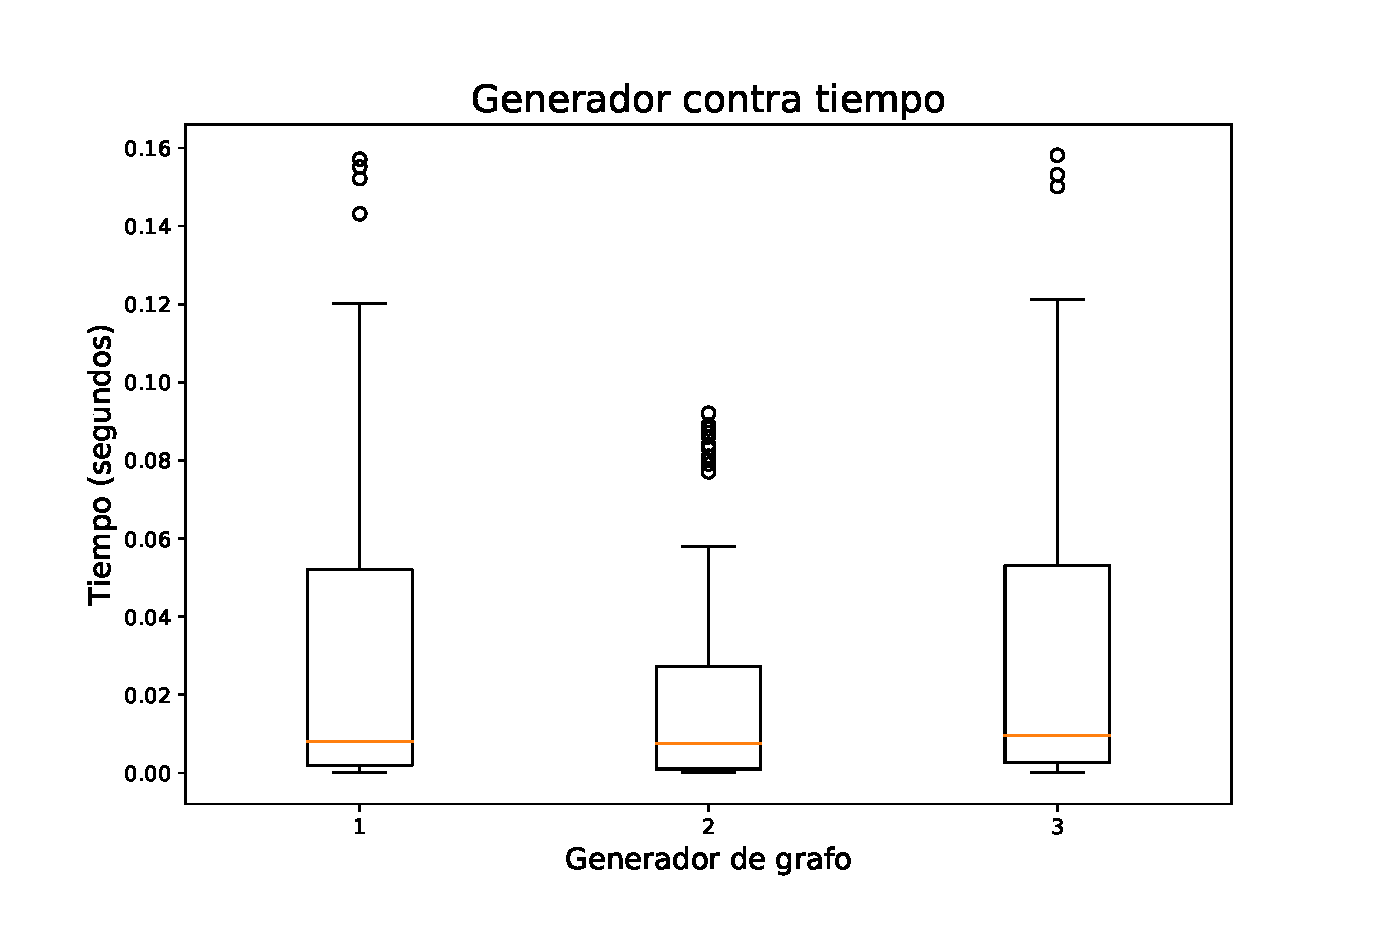
\includegraphics[width=100mm]{boxplotgenerador}
\caption{Tipo de generador de grafo contra tiempo} \label{figure1}
\end{figure}
En la figura \ref{figure1} se puede apreciar que el generador más rápido de los tres seleccionados es el Generador 2, mientras que los otros dos parecen ser igual de tardados.


\subsection*{\centering{Efecto que el algoritmo usado tiene en el tiempo de ejecución}}
\begin{figure}[H]
\centering
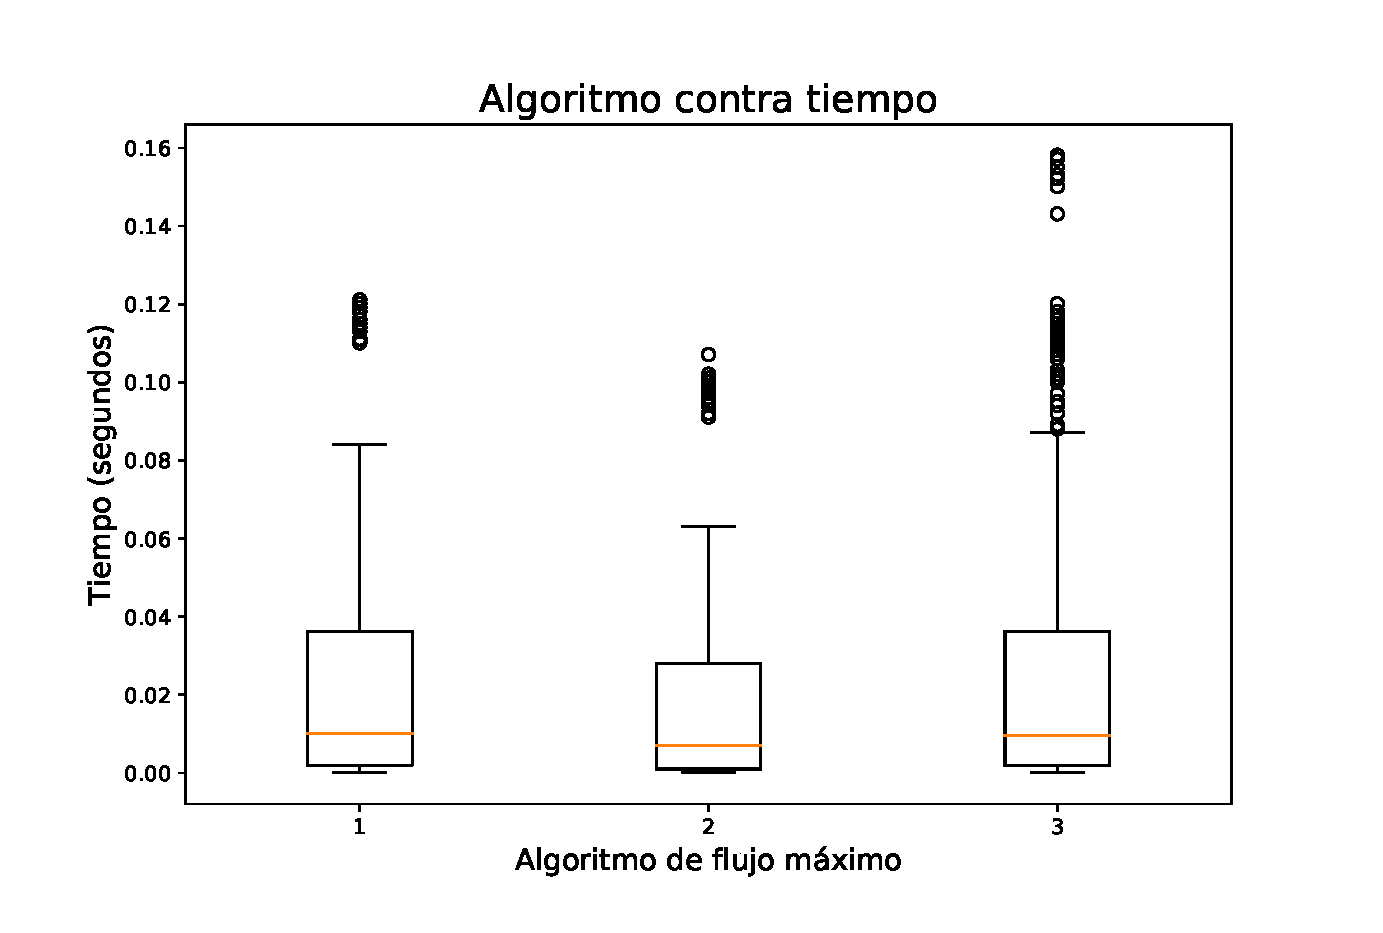
\includegraphics[width=100mm]{boxplotalgoritmo}
\caption{Algoritmo de flujo máximo contra tiempo} \label{figure2}
\end{figure}
En la figura \ref{figure2} se puede apreciar que el algoritmo más rápido de los tres seleccionados es el Algoritmo 2, mientras que el Algoritmo 3 parece ser el más tardado de los tres.


\subsection*{\centering{Efecto que el orden del grafo tiene en el tiempo de ejecución}}
\begin{figure}[H]
\centering
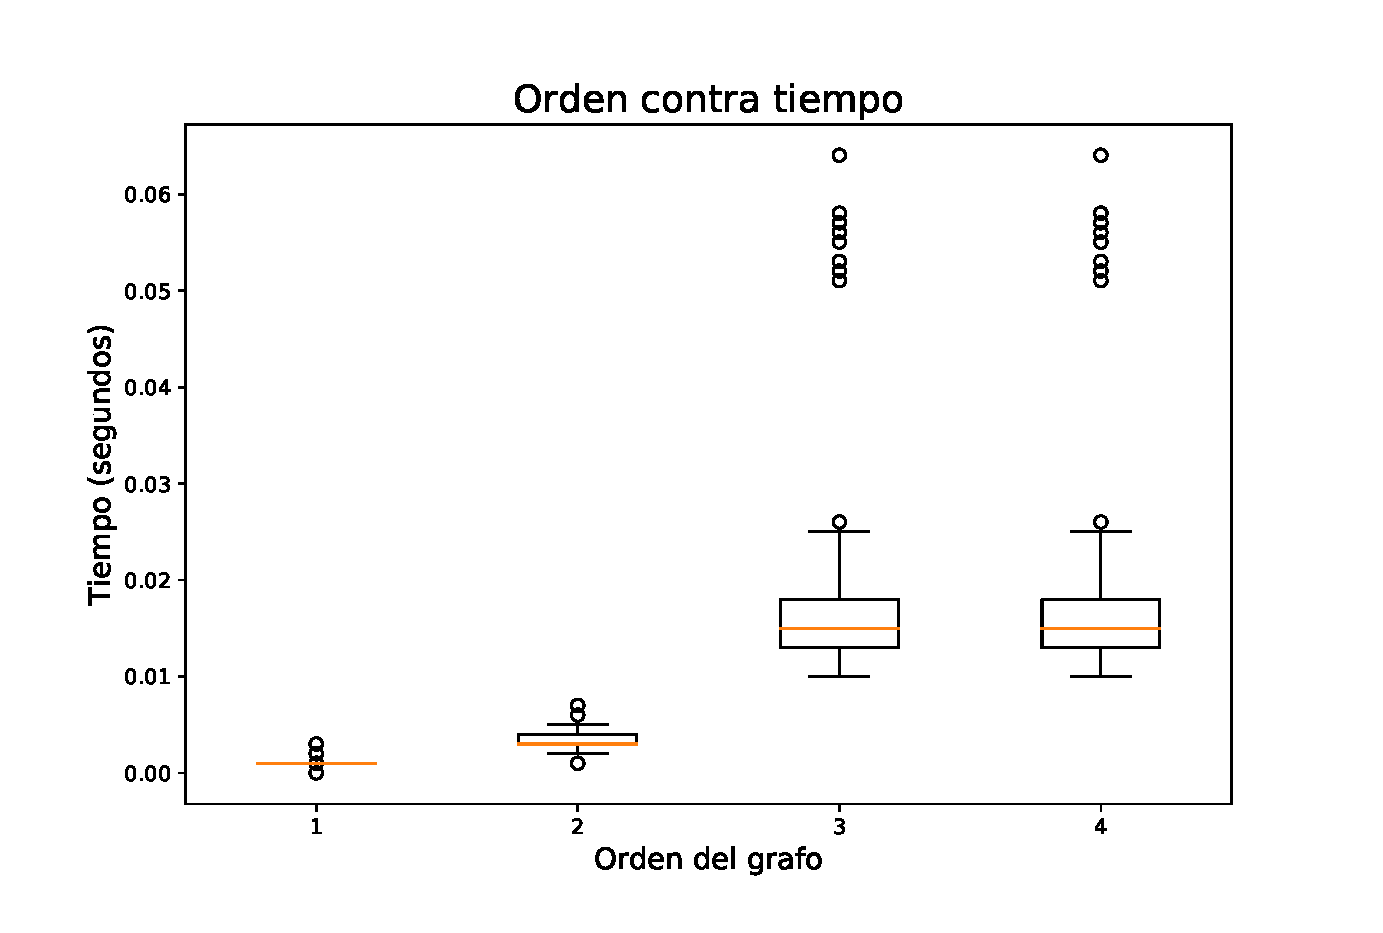
\includegraphics[width=100mm]{boxplotorden}
\caption{Orden del grafo contra tiempo} \label{figure3}
\end{figure}
En la figura \ref{figure3} se puede apreciar que conforme el orden del grafo va creciendo $(2^{4}, 2^{5},  2^{6},  2^{7})$ respectivamente, el tiempo de ejecución también va creciendo.


\subsection*{\centering{Efecto que la densidad del grafo (como tasa de aristas presentes entre aristas posibles) tiene en el tiempo de ejecución}}
\begin{figure}[H]
\centering
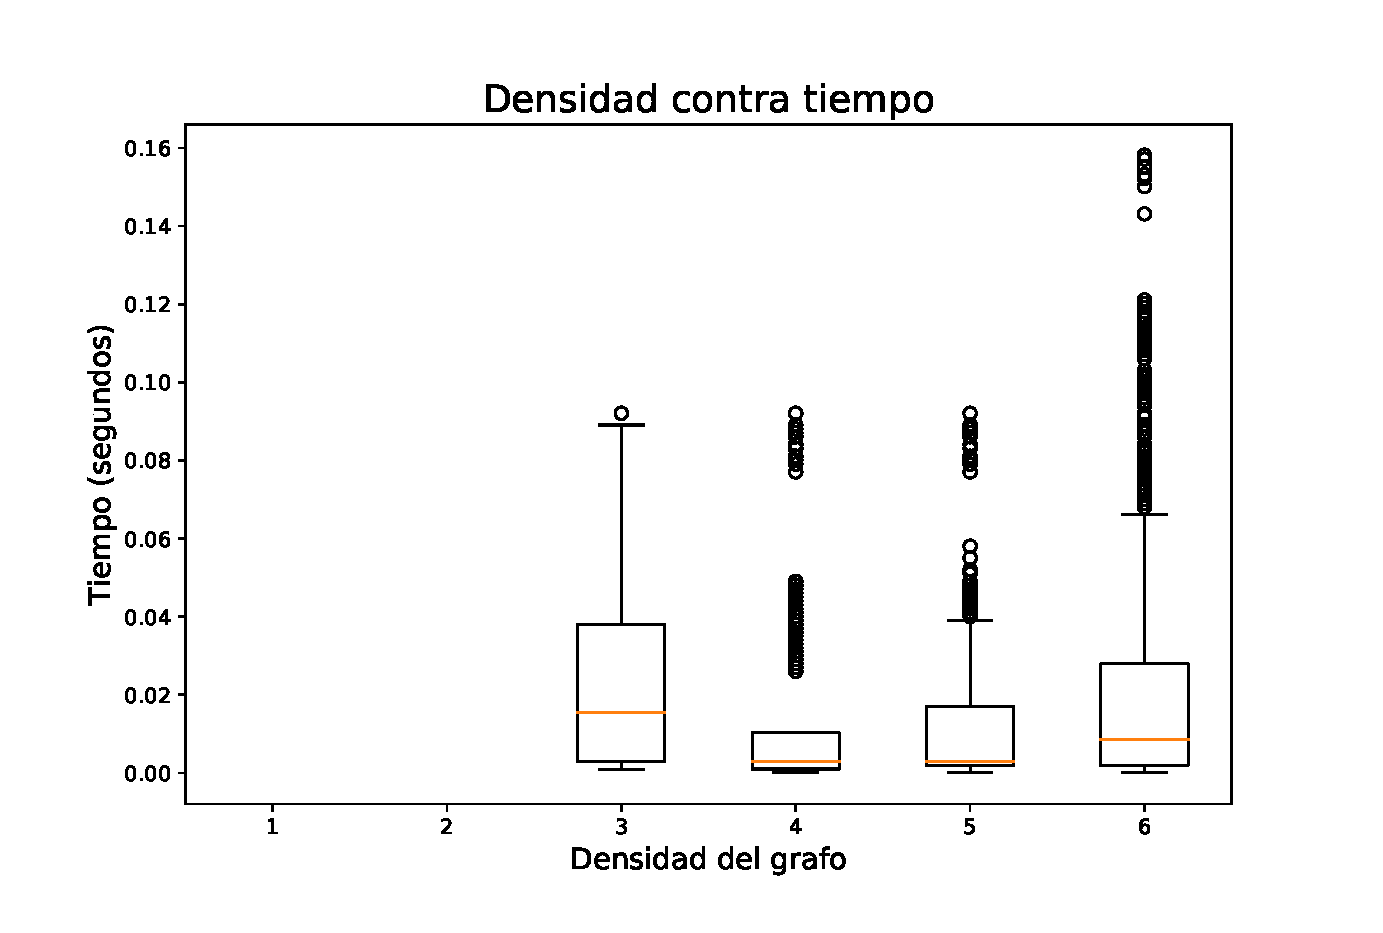
\includegraphics[width=100mm]{boxplotdensidad}
\caption{Densidad del grafo contra tiempo} \label{figure4}
\end{figure}
En la figura \ref{figure4} se puede apreciar que conforme la densidad del grafo va creciendo ([0, 0.5], (0.5, 0.6], (0.6, 0.7],  (0.7, 0.8], (0.8, 0.9], (0.9, 1]) respectivamente, el tiempo de ejecución va disminuyendo.
\\
\\
Se puede observar que los diagramas de caja y bigotes de las figuras \ref{figure1}, \ref{figure2}, \ref{figure3} y \ref{figure4}, no muestran tan profundamente si sí o no estos efectos tienen interacciones, por lo que se sigue a realizar un análisis de varianza para cada una de las variables.
\RecustomVerbatimCommand{\VerbatimInput}{VerbatimInput}
{fontsize=\footnotesize,
 frame=lines,
 framesep=1em, 
 rulecolor=\color{Gray},
 label=\fbox{\color{Black}ANOVA.txt},
 labelposition=topline,
 commandchars=\|\(\),
 commentchar=*  
}
\VerbatimInput{Anova.txt}

Tenemos que el p-valor obtenido por la prueba ANOVA es muy pequeño, es decir, que las medias de las variables con respecto al tiempo son distintas, entonces se puede decir que las variables están relacionadas con los tiempos de ejecución. Una vez hecha la ANOVA se debe verificar que todos los datos deben distribuirse normalmente para que la estadística $F$ sea confiable.


\begin{figure}[H]
\centering
\subfigure[Generador 1]{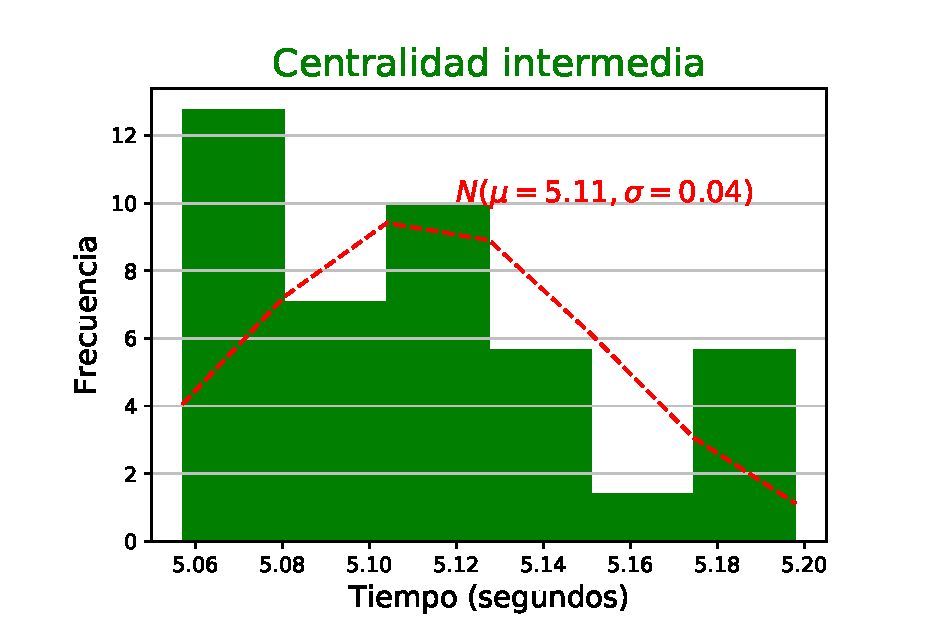
\includegraphics[width=80mm]{./histograma1}}
\subfigure[Generador 2]{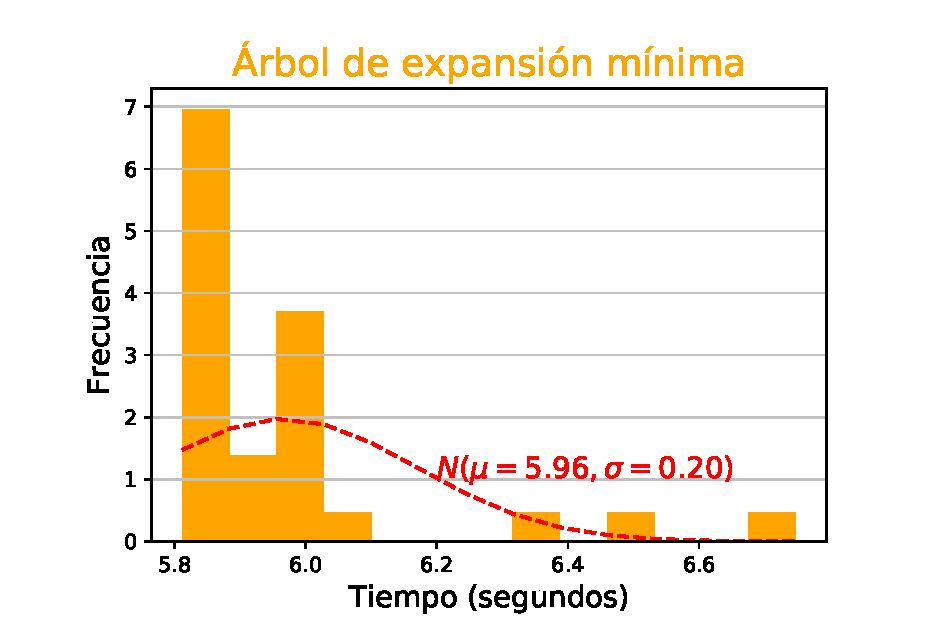
\includegraphics[width=80mm]{./histograma2}}
\subfigure[Generador 3]{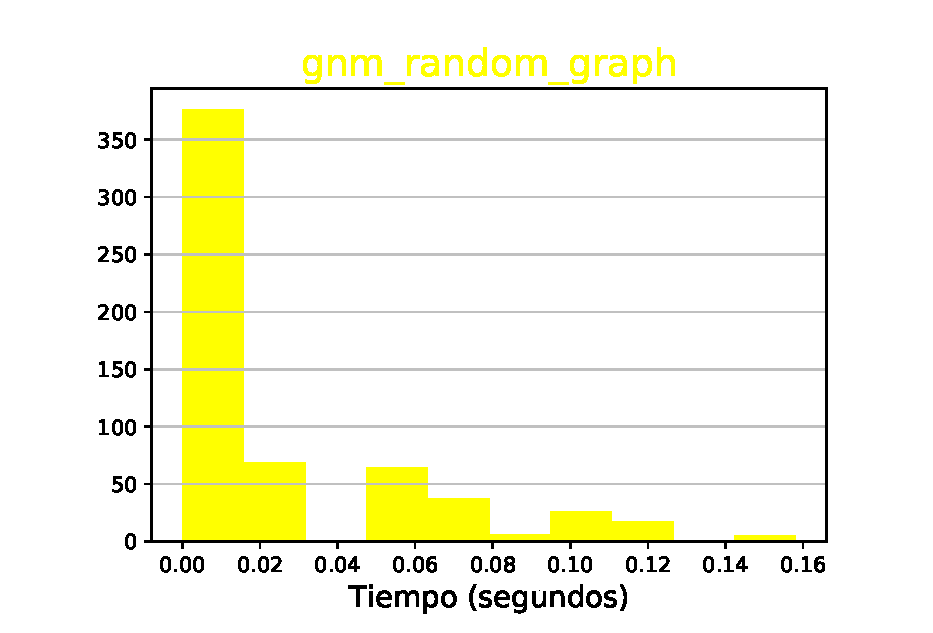
\includegraphics[width=80mm]{./histograma3}}
\caption{Histogramas de los tiempos por tipo de generador de grafo} \label{figure5}
\end{figure}

De la figura \ref{figure5} es fácil ver que los datos de los tiempos de los generados de grafos no son distribuidos normalmente.


\begin{figure}[H]
\centering
\subfigure[Algoritmo 1]{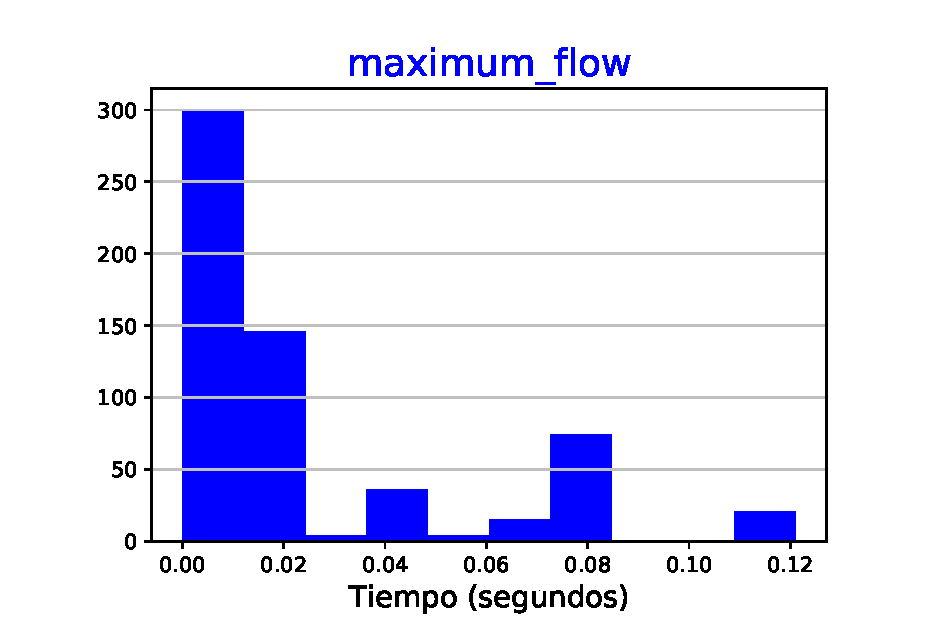
\includegraphics[width=80mm]{./histograma4}}
\subfigure[Algoritmo 2]{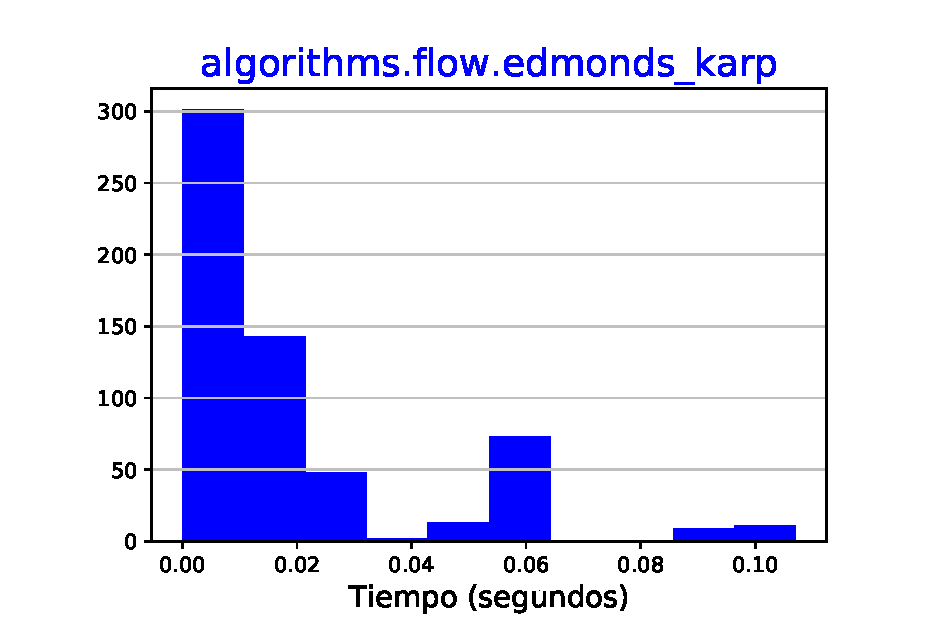
\includegraphics[width=80mm]{./histograma5}}
\subfigure[Algoritmo 3]{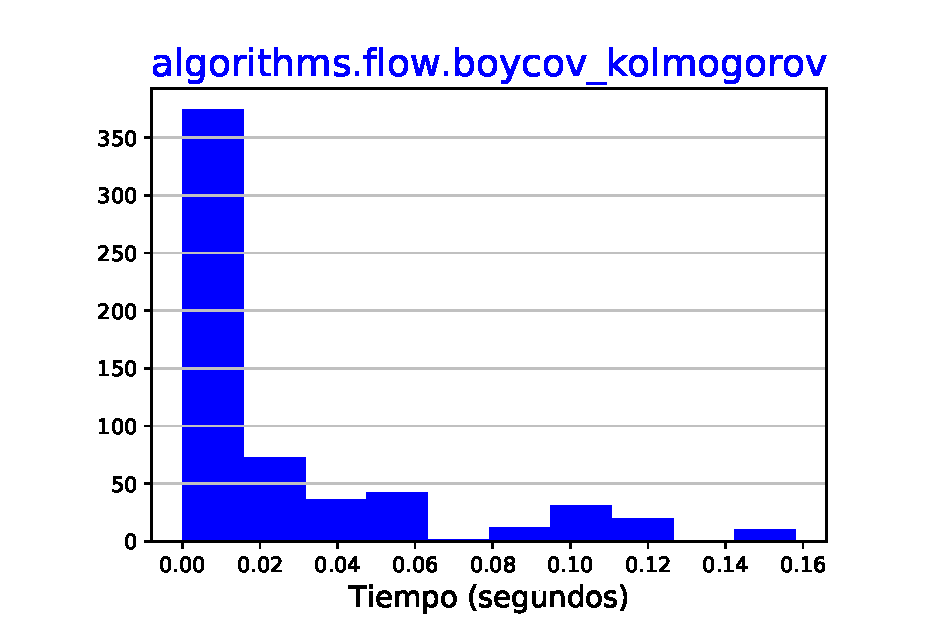
\includegraphics[width=80mm]{./histograma6}}
\caption{Histogramas de los tiempos por tipo de algoritmo de flujo máximo} \label{figure6}
\end{figure}

De la figura \ref{figure6} es fácil ver que los datos de los tiempos de los algoritmos de flujo máximo no son distribuidos normalmente.


\begin{figure}[H]
\centering
\subfigure[Orden (16)]{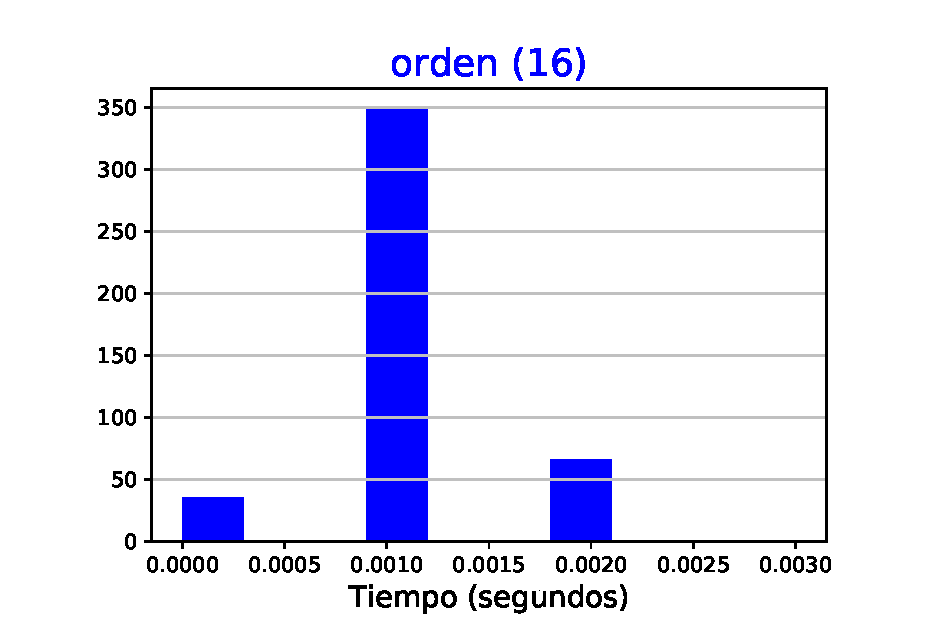
\includegraphics[width=80mm]{./histograma7}}
\subfigure[Orden (32)]{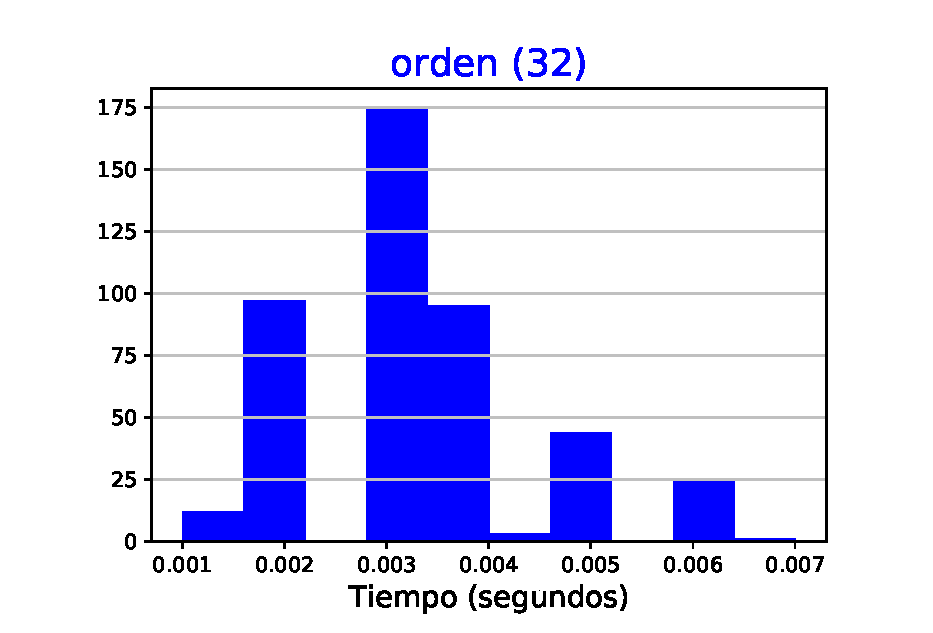
\includegraphics[width=80mm]{./histograma8}}
\subfigure[Orden (64)]{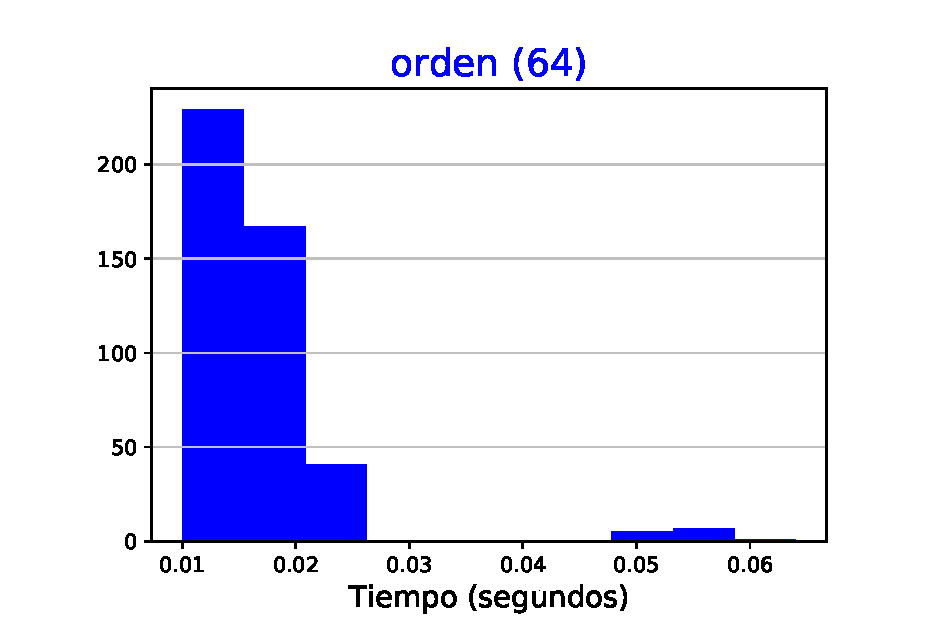
\includegraphics[width=80mm]{./histograma9}}
\subfigure[Orden (128)]{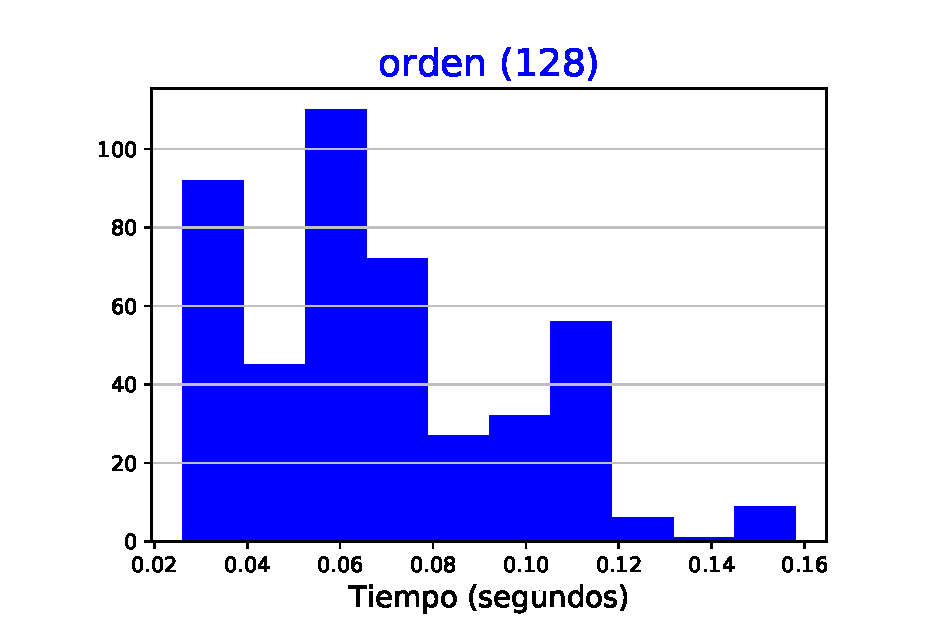
\includegraphics[width=80mm]{./histograma10}}
\caption{Histogramas de los tiempos por tamaño de orden del grafo} \label{figure7}
\end{figure}

De la figura \ref{figure7} es fácil ver que los datos de los tiempos por tamaño del orden de los grafos no son distribuidos normalmente.
\\
\\
De las figuras \ref{figure5}, \ref{figure6}, y \ref{figure7}, podemos ver que los tiempos de ejecución no distribuyen normalmente para las variables por lo que se propone para estudiar más a fondo la relación entre las variables una prueba de Mínimos Cuadrados (OLS).
\newpage
\RecustomVerbatimCommand{\VerbatimInput}{VerbatimInput}
{fontsize=\footnotesize,
 frame=lines,
 framesep=1em, 
 rulecolor=\color{Gray},
 label=\fbox{\color{Black}OLS.txt},
 labelposition=topline,
 commandchars=\|\(\),
 commentchar=*  
}
\VerbatimInput{Ols.txt}

La prueba de Mínimos Cuadros muestra con la $r-cuadrada$ que se puede eliminar hasta el 75\% de errores para determinar el tiempo, por otro lado, el $p-valor$ muestra que la medias de las variables son distintas respecto al tiempo y por último podemos ver que la variable Orden está más relacionada con los tiempos de ejecución, luego le sigue el Densidad del grafo y déspues el Algoritmo de flujo máximo. Para rectificar la prueba de Mínimos Cuadrados se hace una Matriz de Correlaciones. Ver figura \ref{figure8}.




\begin{figure}[H]
\centering
\includegraphics[width=100mm]{Correlaciones}
\caption{Matriz de correlaciones} \label{figure8}
\end{figure}

Por último se representan en la figura \ref{figure9} todos los grafos y se identifican según su generador por color y su algorimo de solución por forma.
\begin{figure}[H]
\centering
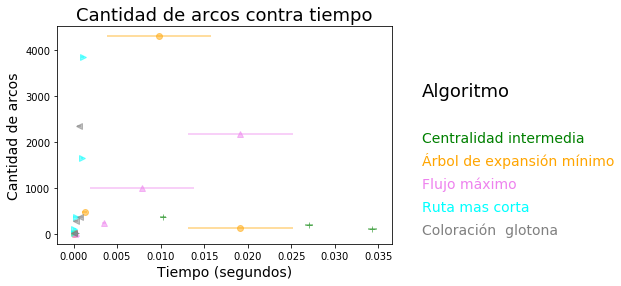
\includegraphics[width=170mm]{imagen2}
\caption{Grafos contra tiempo} \label{figure9}
\end{figure}


\bibliographystyle{unsrt}
\bibliography{biblio}
\nocite{*}

\end{document}